% !TeX program = xelatex
\documentclass[a4paper,10pt]{article}

% ============================================================================
% សន្លឹកកិច្ចការសិស្ស ស-ខ្មៅ (Student Guided-Inquiry Worksheet - Grade 8 13.2.1a PARA1)
% បរិបទ៖ ថ្នាក់រៀនគ្មានស្លាយ LCD – វាស់ពិនិត្យ និងបំពេញតារាងសម្រាយបញ្ជាក់បន្ថយជំនួយ ២ ទំព័រ A4
% ============================================================================
\usepackage[a4paper, left=0.90cm, right=0.90cm, top=0.75cm, bottom=0.85cm, footskip=0.45cm]{geometry}
\usepackage{amsmath, amssymb}
\usepackage{unicode-math}
\usepackage{fontspec}
\usepackage{array, colortbl}
\usepackage[table]{xcolor}
\usepackage{enumitem}
\usepackage{pifont}
\usepackage{fancyhdr}
\usepackage{lastpage}
\usepackage{tikz}
\usepackage[most]{tcolorbox}
\usetikzlibrary{calc, arrows.meta, angles, quotes, decorations.markings, positioning, babel}

\makeatletter
\let\@expl@@@mark@update@singlecol@structures@@\relax
\makeatother

\providecommand{\NGSFindFonts}{%
  \IfFileExists{C:/Windows/Fonts/cambria.ttc}{%
    \def\NGSSysPath{C:/Windows/Fonts/}%
    \def\NGSUserPath{C:/Users/KIT/AppData/Local/Microsoft/Windows/Fonts/}%
  }{%
    \IfFileExists{./fonts/KhmerOSsiemreap.ttf}{\def\NGSSysPath{./fonts/}\def\NGSUserPath{./fonts/}}{%
    \IfFileExists{../fonts/KhmerOSsiemreap.ttf}{\def\NGSSysPath{../fonts/}\def\NGSUserPath{../fonts/}}{%
    \IfFileExists{../../fonts/KhmerOSsiemreap.ttf}{\def\NGSSysPath{../../fonts/}\def\NGSUserPath{../../fonts/}}{%
    \IfFileExists{../../../fonts/KhmerOSsiemreap.ttf}{\def\NGSSysPath{../../../fonts/}\def\NGSUserPath{../../../fonts/}}{%
    \IfFileExists{../../../../fonts/KhmerOSsiemreap.ttf}{\def\NGSSysPath{../../../../fonts/}\def\NGSUserPath{../../../../fonts/}}{%
    \IfFileExists{../../../../../fonts/KhmerOSsiemreap.ttf}{\def\NGSSysPath{../../../../../fonts/}\def\NGSUserPath{../../../../../fonts/}}{%
    \IfFileExists{../../../../../../fonts/KhmerOSsiemreap.ttf}{\def\NGSSysPath{../../../../../../fonts/}\def\NGSUserPath{../../../../../../fonts/}}{%
      \def\NGSSysPath{../../../../../../../fonts/}\def\NGSUserPath{../../../../../../../fonts/}%
    }}}}}}}%
  }%
}
\NGSFindFonts

\setmathfont[Path={\NGSSysPath}, FontIndex=1, Scale=1.02]{cambria.ttc}
\defaultfontfeatures{Ligatures=TeX}

\setmainfont[
  Path={\NGSUserPath},
  Extension=.ttf,
  Script=Khmer,
  BoldFont={KhmerOSsiemreap},
  BoldFeatures={FakeBold=1.8},
  ItalicFont={KhmerOSsiemreap},
  ItalicFeatures={FakeSlant=0.25},
  BoldItalicFont={KhmerOSsiemreap},
  BoldItalicFeatures={FakeBold=1.8, FakeSlant=0.25}
]{KhmerOSsiemreap}

\newfontfamily\muol[Path={\NGSUserPath}, Extension=.ttf, Script=Khmer]{KhmerOSmuollight}
\newfontfamily\TimesEn[Path={\NGSSysPath}, Extension=.ttf, BoldFont={timesbd}, ItalicFont={timesi}, BoldItalicFont={timesbi}]{times}

\XeTeXlinebreaklocale "km"
\XeTeXlinebreakskip = 0pt plus 1pt minus 0.1pt

\definecolor{panelgray}{gray}{0.94}
\definecolor{headgray}{gray}{0.86}
\definecolor{subgray}{gray}{0.91}

\pagestyle{fancy}
\fancyhf{}
\renewcommand{\headrulewidth}{0pt}
\fancyfoot[L]{\fontsize{8pt}{10pt}\selectfont អនុវិទ្យាល័យព្រះក្រសាំង \en{|} គណិតវិទ្យា ថ្នាក់ទី៨ \en{|} មេរៀនទី១៣ (២.១.១ លក្ខណៈប្រលេឡូក្រាម៖ ទ្រឹស្ដីបទទី១--៣)}
\fancyfoot[R]{\fontsize{8.2pt}{10pt}\selectfont ទំព័រ \en{\thepage\ / \pageref{LastPage}}}

\setlength{\parindent}{0pt}
\setlength{\parskip}{0pt}
\setlength{\tabcolsep}{4pt}

\newcommand{\en}[1]{{\TimesEn #1}}
\newcommand{\enbf}[1]{{\TimesEn\textbf{#1}}}
\newcommand{\unit}[1]{\,\text{\en{#1}}}
\newcommand{\cnum}[1]{{\fontsize{10pt}{12pt}\selectfont\ding{\numexpr171+#1\relax}}}
\newcommand{\chk}{\tikz[baseline=-0.15ex]\draw[black, line width=0.8pt] (0,0) rectangle (0.25cm,0.25cm);}
\newcommand{\tri}[1]{\ensuremath{\triangle #1}}
\newcommand{\ang}[1]{\ensuremath{\angle #1}}
\newcommand{\cg}{\ensuremath{\cong}}
\newcommand{\dotline}[1]{\makebox[#1]{\dotfill}}

\newcolumntype{L}[1]{>{\raggedright\arraybackslash}p{#1}}
\newcolumntype{C}[1]{>{\centering\arraybackslash}p{#1}}

\tikzset{
  tk1/.style={postaction={decorate},decoration={markings,mark=at position 0.50 with {\draw[black, line width=0.95pt](0,-0.10)--(0,0.10);}}},
  tk2/.style={postaction={decorate},decoration={markings,
    mark=at position 0.45 with {\draw[black, line width=0.95pt](0,-0.10)--(0,0.10);},
    mark=at position 0.55 with {\draw[black, line width=0.95pt](0,-0.10)--(0,0.10);}}},
  par1/.style={postaction={decorate},decoration={markings,mark=at position 0.52 with {\draw[black, line width=0.95pt](-0.07,0.08)--(0.05,0)--(-0.07,-0.08);}}},
  par2/.style={postaction={decorate},decoration={markings,
    mark=at position 0.46 with {\draw[black, line width=0.95pt](-0.07,0.08)--(0.05,0)--(-0.07,-0.08);},
    mark=at position 0.58 with {\draw[black, line width=0.95pt](-0.07,0.08)--(0.05,0)--(-0.07,-0.08);}}}
}

\newcommand{\secbar}[2]{%
  \vspace{3pt}
  \noindent\colorbox{headgray}{\parbox{\dimexpr\linewidth-2\fboxsep\relax}{%
    \vspace{1.5pt}{\muol\fontsize{9.5pt}{13.5pt}\selectfont #1}\hfill{\fontsize{8.5pt}{12pt}\selectfont\textbf{#2}}\vspace{1.5pt}%
  }}\par\vspace{3pt}
}

\begin{document}
\fontsize{9.5pt}{14.4pt}\selectfont

% ============================================================================
% ទំព័រទី១៖ E1 ទស្សន៍ទាយ + E2 វាស់ខ្នាតពិត 1:1 & តារាងសម្រាយបញ្ជាក់បន្ថយជំនួយ
% ============================================================================
\begin{tcolorbox}[enhanced, sharp corners, colback=white, colframe=black, boxrule=1.0pt, top=4pt, bottom=4pt, left=6pt, right=6pt]
  \begin{center}
    {\muol\fontsize{10.5pt}{15pt}\selectfont សន្លឹកកិច្ចការសិស្ស — មេរៀនទី១៣៖ ចតុកោណ \enbf{(}២.១.១ លក្ខណៈប្រលេឡូក្រាម\enbf{)}}\\[2pt]
    {\footnotesize សៀវភៅសិក្សាគោលថ្នាក់ទី៨ ទំព័រ ១៧០--១៧១ និង ១៨៥ \en{|} វាស់ពិនិត្យ និងបំពេញតារាងសម្រាយបញ្ជាក់ (គ្មានស្លាយ \en{LCD})}
  \end{center}
  \vspace{2pt}
  \hrule height 0.5pt
  \vspace{4pt}
  ឈ្មោះសិស្សទី១៖ \dotline{3.6cm} \hspace{0.15cm} ឈ្មោះដៃគូទី២៖ \dotline{3.6cm} \hspace{0.15cm} ថ្នាក់ទី៨៖ \dotline{1.0cm} \hspace{0.15cm} ថ្ងៃទី១២/១២/២០២៦
\end{tcolorbox}

% --- E1 Engage ---
\secbar{ផ្នែកទី១ ៖ បេសកកម្មផ្ដើមមេរៀន — ជន្ទល់កន្ត្រៃលើកទំនិញ \enbf{(E1 -- Engage)}}{៣ នាទី}
\begin{tcolorbox}[enhanced, sharp corners, colback=panelgray, colframe=black, boxrule=0.7pt, top=3.5pt, bottom=3.5pt, left=6pt, right=6pt]
  \textbf{ស្ថានភាពពិត៖} ស៊ុមជន្ទល់កន្ត្រៃរាងប្រលេឡូក្រាម $ABCD$ ($AB\parallel DC, AD\parallel BC$) មានដែកទ្រូង $AC$ និង $BD$ ប្រសព្វគ្នាត្រង់ប៊ូឡុង $O$ ។\par\vspace{2pt}
  $\bullet$ \textbf{កូនជាង ក ថា៖} «ជ្រុងឈមស្មើគ្នា ($AB=DC, AD=BC$) ហើយដែកទ្រូងទាំងពីរក៏ស្មើគ្នាដែរ ($AC=BD$)!»\par
  $\bullet$ \textbf{កូនជាង ខ ថា៖} «ពេលទ្រេត $AC \neq BD$ ទេ ប៉ុន្តែប៊ូឡុង $O$ ចែកអង្កត់ទ្រូងនីមួយៗជាពីរស្មើគ្នា ($OA=OC$ និង $OB=OD$)!»\par\vspace{2pt}
  \textbf{ការទស្សន៍ទាយដំបូងរបស់ដៃគូអ្នក៖} \hspace{0.3cm} \chk\ គាំទ្រកូនជាង ក \hspace{0.6cm} \chk\ គាំទ្រកូនជាង ខ \hspace{0.6cm} \chk\ មិនទាន់ប្រាកដ
\end{tcolorbox}

% --- E2 Explore ---
\secbar{ផ្នែកទី២ ៖ ពិសោធន៍វាស់ខ្នាតពិត \enbf{1:1} និងតារាងសម្រាយបញ្ជាក់បន្ថយជំនួយ \enbf{(E2 -- Explore)}}{១១ នាទី}
\textbf{សកម្មភាពទី១ (៥.៥ នាទី)៖} ប្រើ\textbf{បន្ទាត់ក្រិត} និង\textbf{រ៉ាប់ព័រទ័រ} វាស់ប្រលេឡូក្រាមខ្នាតពិត $ABCD$ ($AB=5.0\unit{cm}, AD=3.2\unit{cm}, \ang{D}=60^\circ$) ខាងឆ្វេង រួចបំពេញតារាងខាងស្ដាំ៖

\vspace{3pt}
\begin{tabular}{@{}C{7.55cm} L{11.15cm}@{}}
  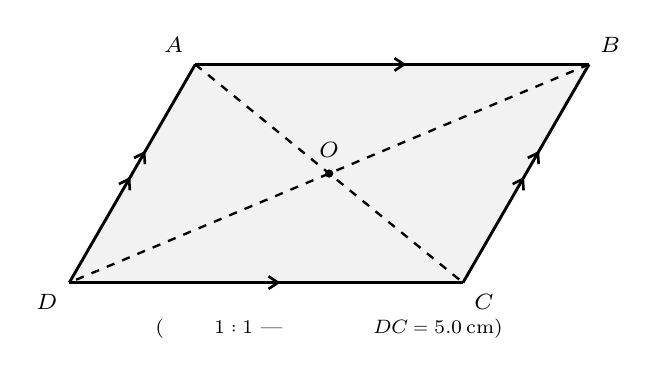
\begin{tikzpicture}[x=1cm, y=1cm, baseline={(0,1.45)}, every node/.style={font=\footnotesize, text=black}]
    % True 1:1 parallelogram: D=(0,0), C=(5.0,0), A=(1.60,2.771), B=(6.60,2.771) -> AD = 3.20 cm, angle D = 60 deg!
    \coordinate (D) at (0,0);
    \coordinate (C) at (5.00,0);
    \coordinate (A) at (1.60,2.771);
    \coordinate (B) at (6.60,2.771);
    \coordinate (O) at ($(A)!0.5!(C)$);
    \fill[gray!10] (A)--(B)--(C)--(D)--cycle;
    \draw[black, line width=1.05pt, par1] (A)--(B);
    \draw[black, line width=1.05pt, par1] (D)--(C);
    \draw[black, line width=1.05pt, par2] (D)--(A);
    \draw[black, line width=1.05pt, par2] (C)--(B);
    \draw[black, line width=0.85pt, dashed] (A)--(C) (B)--(D);
    \fill[black] (O) circle (1.5pt) node[above=2pt] {$O$};
    \node[above left=1pt] at (A) {$A$};
    \node[above right=1pt] at (B) {$B$};
    \node[below right=1pt] at (C) {$C$};
    \node[below left=1pt] at (D) {$D$};
    \node[font=\scriptsize] at (3.30,-0.58) {(ខ្នាតពិត $1:1$ — ផ្ទៀងបន្ទាត់លើ $DC=5.0\unit{cm}$)};
  \end{tikzpicture}
  &
  {\renewcommand{\arraystretch}{1.34}
  \begin{tabular}{|L{4.85cm}|L{5.65cm}|}
    \hline
    \rowcolor{subgray}\textbf{ធាតុដែលត្រូវវាស់} & \textbf{លទ្ធផលវាស់ និងការសង្កេត} \\
    \hline
    ជ្រុងឈមទី១៖ $AB$ និង $DC$ & $AB=\dotline{1.2cm}$, $DC=\dotline{1.2cm}$ \\
    \hline
    ជ្រុងឈមទី២៖ $AD$ និង $BC$ & $AD=\dotline{1.2cm}$, $BC=\dotline{1.2cm}$ \\
    \hline
    មុំឈម៖ $\ang{D}, \ang{B}$ និង $\ang{A}, \ang{C}$ & $\ang{D}=\dotline{1.0cm}, \ang{B}=\dotline{1.0cm}, \ang{A}=\dotline{1.0cm}$ \\
    \hline
    ផលបូកមុំជាប់៖ $\ang{A}+\ang{B}$ & $\ang{A}+\ang{B}=\dotline{2.2cm}^\circ$ \\
    \hline
    អង្កត់ទ្រូងពេញ៖ $AC$ និង $BD$ & $AC\approx\dotline{1.1cm}$, $BD\approx\dotline{1.1cm}$ (\chk\ ស្មើ \chk\ មិនស្មើ) \\
    \hline
    កំណាត់ពី $O$៖ $OA, OC$ និង $OB, OD$ & $OA=\dotline{1.0cm}=OC$; $OB=\dotline{1.0cm}=OD$ \\
    \hline
  \end{tabular}}
\end{tabular}

\vspace{6pt}
\textbf{សកម្មភាពទី២ — តារាងសម្រាយបញ្ជាក់បន្ថយជំនួយ (\en{Faded Proof Table}, ៥.៥ នាទី)៖} គូសសញ្ញាធ្នូមុំឆ្លាស់ក្នុង និងព័ទ្ធរង្វង់ជ្រុងរួមលើរូប រួចបំពេញចន្លោះ៖

\vspace{4pt}
{\renewcommand{\arraystretch}{1.32}
\begin{tabular}{|L{9.10cm}|L{9.10cm}|}
  \hline
  \rowcolor{headgray}
  \textbf{ផ្នែក ក៖ ទ្រឹស្ដីបទទី១--២ (គូសអង្កត់ទ្រូង $AC$ ១ ខ្សែ)} &
  \textbf{ផ្នែក ខ៖ ទ្រឹស្ដីបទទី៣ (អង្កត់ទ្រូង $AC \cap BD = \{O\}$)} \\
  \hline
  \begin{center}
  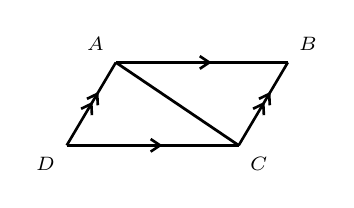
\begin{tikzpicture}[scale=0.78, every node/.style={font=\scriptsize}]
    \coordinate (D) at (0,0); \coordinate (C) at (2.8,0);
    \coordinate (A) at (0.8,1.35); \coordinate (B) at (3.6,1.35);
    \draw[line width=0.95pt, par1] (A)--(B); \draw[line width=0.95pt, par1] (D)--(C);
    \draw[line width=0.95pt, par2] (D)--(A); \draw[line width=0.95pt, par2] (C)--(B);
    \draw[line width=1.0pt] (A)--(C);
    \node[above left=1pt] at (A) {$A$}; \node[above right=1pt] at (B) {$B$};
    \node[below right=1pt] at (C) {$C$}; \node[below left=1pt] at (D) {$D$};
  \end{tikzpicture}
  \end{center}
  ប្រៀបធៀប $\tri{ADC}$ និង $\tri{ABC}$ មាន៖\par
  ១. $\ang{DAC} = \ang{\dotline{1.1cm}}$ (មុំឆ្លាស់ក្នុងនៃ $AD \parallel BC$)\par
  ២. $AC$ ជាជ្រុង \dotline{2.0cm} (ព័ទ្ធរង្វង់ \textbf{[tracing]})\par
  ៣. $\ang{DCA} = \ang{\dotline{1.1cm}}$ (មុំឆ្លាស់ក្នុងនៃ $AB \parallel DC$)\par
  $\Rightarrow \tri{ADC} \cg \tri{ABC}$ តាមលក្ខណៈ \textbf{(\dotline{1.5cm})} ។\par
  $\bullet$ \textbf{វិបាក៖} ជ្រុងឈម $AD=\dotline{1.0cm}, AB=\dotline{1.0cm}$ និងមុំឈម $\ang{D}=\ang{\dotline{0.8cm}}$\par
  $\bullet$ ដោយ $AD\parallel BC$ កាត់ដោយ $AB$ នោះ $\ang{A}+\ang{B} = \dotline{1.3cm}^\circ$ ។
  &
  \begin{center}
  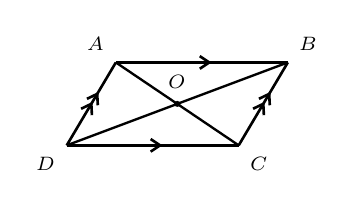
\begin{tikzpicture}[scale=0.78, every node/.style={font=\scriptsize}]
    \coordinate (D) at (0,0); \coordinate (C) at (2.8,0);
    \coordinate (A) at (0.8,1.35); \coordinate (B) at (3.6,1.35);
    \coordinate (O) at ($(A)!0.5!(C)$);
    \draw[line width=0.95pt, par1] (A)--(B); \draw[line width=0.95pt, par1] (D)--(C);
    \draw[line width=0.95pt, par2] (D)--(A); \draw[line width=0.95pt, par2] (C)--(B);
    \draw[line width=0.85pt] (A)--(C) (B)--(D);
    \fill (O) circle (1.4pt) node[above=2pt] {$O$};
    \node[above left=1pt] at (A) {$A$}; \node[above right=1pt] at (B) {$B$};
    \node[below right=1pt] at (C) {$C$}; \node[below left=1pt] at (D) {$D$};
  \end{tikzpicture}
  \end{center}
  ប្រៀបធៀប $\tri{AOB}$ និង $\tri{COD}$ មាន៖\par
  ១. $\ang{OAB} = \ang{\dotline{1.1cm}}$ (មុំឆ្លាស់ក្នុងនៃ $AB \parallel DC$)\par
  ២. ជ្រុង $AB = \dotline{1.2cm}$ (ជ្រុងឈមប្រលេឡូក្រាមស្មើគ្នា)\par
  ៣. $\ang{OBA} = \ang{\dotline{1.1cm}}$ (មុំឆ្លាស់ក្នុងនៃ $AB \parallel DC$)\par
  $\Rightarrow \tri{AOB} \cg \tri{COD}$ តាមលក្ខណៈ \textbf{(\dotline{1.5cm})} ។\par
  $\bullet$ \textbf{ធាតុត្រូវគ្នា៖} $OA = \dotline{1.1cm}$ និង $OB = \dotline{1.1cm}$ ។\par
  $\bullet$ ដូច្នេះ ចំណុចប្រសព្វ $O$ ជាចំណុច \dotline{2.0cm} នៃអង្កត់ទ្រូងទាំងពីរ ។ \\
  \hline
\end{tabular}}

% ============================================================================
% ទំព័រទី២៖ E3 ធនាគារហេតុផល + E4 លំហាត់គំរូ + E5 ប្រតិបត្តិ & Exit + កិច្ចការផ្ទះ
% ============================================================================
\newpage

\secbar{ផ្នែកទី៣ ៖ សង្ខេបទ្រឹស្ដីបទទី១--៣ និងធនាគារហេតុផល \cnum{1}\enbf{--}\cnum{5} \enbf{(E3 -- Explain)}}{៦ នាទី}
\begin{tcolorbox}[enhanced, sharp corners, colback=white, colframe=black, boxrule=0.75pt, top=4pt, bottom=4pt, left=6pt, right=6pt]
  \cnum{1}\ \textbf{និយមន័យ៖} ប្រលេឡូក្រាមមានជ្រុងឈមស្របគ្នាពីរៗ ($AB\parallel DC$ និង $AD\parallel BC$) ។\par\vspace{2pt}
  \cnum{2}\ \textbf{ទ្រឹស្ដីបទទី១៖} អង្កត់ទ្រូងនីមួយៗចែកប្រលេឡូក្រាមជាត្រីកោណពីរ \dotline{2.0cm} ($\tri{ADC}\cg\tri{ABC}$) ។\par\vspace{2pt}
  \cnum{3}\ \textbf{វិបាកទ្រឹស្ដីបទទី១៖} ក្នុងប្រលេឡូក្រាម ជ្រុងឈម \dotline{1.8cm} ពីរៗ ($AB=DC, AD=BC$) និងមុំឈម \dotline{1.8cm} ពីរៗ ($\ang{A}=\ang{C}, \ang{B}=\ang{D}$) ។\par\vspace{2pt}
  \cnum{4}\ \textbf{ទ្រឹស្ដីបទទី២៖} មុំពីរជាប់គ្នានៃប្រលេឡូក្រាមជាមុំ \dotline{2.2cm} ($\ang{A}+\ang{B} = \dotline{1.2cm}^\circ$) ។\par\vspace{2pt}
  \cnum{5}\ \textbf{ទ្រឹស្ដីបទទី៣៖} អង្កត់ទ្រូងទាំងពីរកាត់គ្នាត្រង់ \dotline{2.5cm} នីមួយៗ ($OA=OC, OB=OD$) ហៅថា\textbf{ផ្ចិតឆ្លុះ}នៃប្រលេឡូក្រាម ។
\end{tcolorbox}

% --- E4 Elaborate ---
\secbar{ផ្នែកទី៤ ៖ លំហាត់គំរូអនុវត្ត \enbf{[tracing]} និងធនាគារហេតុផល \cnum{1}\enbf{--}\cnum{5} \enbf{(E4 -- Elaborate)}}{១០ នាទី}
{\renewcommand{\arraystretch}{1.32}
\begin{tabular}{|L{9.10cm}|L{9.10cm}|}
  \hline
  \rowcolor{subgray}
  \textbf{គំរូទី១ (លំហាត់ទី៤ ទំ.១៨៥ — គណនាមុំទាំងបួន)} &
  \textbf{គំរូទី២ (លំហាត់ទី២ ទំ.១៨៥ — អង្កត់កាត់តាមផ្ចិតឆ្លុះ $I$)} \\
  \hline
  គណនារង្វាស់មុំទាំងបួននៃប្រលេឡូក្រាម $ABCD$ ដោយដឹងថារង្វាស់មុំមួយស្មើពីរដងនៃរង្វាស់មុំមួយទៀត ។\par
  \begin{center}
  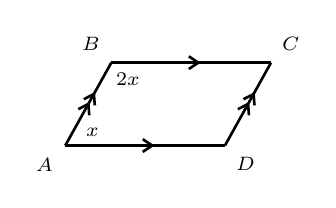
\begin{tikzpicture}[scale=0.78, every node/.style={font=\scriptsize}]
    \draw[line width=0.95pt, par1] (0.75,1.35)--(3.35,1.35);
    \draw[line width=0.95pt, par1] (0,0)--(2.60,0);
    \draw[line width=0.95pt, par2] (0,0)--(0.75,1.35);
    \draw[line width=0.95pt, par2] (2.60,0)--(3.35,1.35);
    \node[below left=1pt] at (0,0) {$A$}; \node[above left=1pt] at (0.75,1.35) {$B$};
    \node[above right=1pt] at (3.35,1.35) {$C$}; \node[below right=1pt] at (2.60,0) {$D$};
    \node at (0.45,0.22) {$x$}; \node at (1.02,1.08) {$2x$};
  \end{tikzpicture}
  \end{center}
  $\bullet$ តាង $\ang{A}=x$ នោះមុំជាប់គ្នា $\ang{B} = \dotline{1.2cm}$\par
  $\bullet$ តាមហេតុផលលេខ \dotline{0.9cm}៖ $\ang{A}+\ang{B}=180^\circ$\par
  $\Rightarrow x + \dotline{1.2cm} = 180^\circ \Rightarrow 3x = 180^\circ \Rightarrow x = \dotline{1.2cm}^\circ$\par
  $\bullet$ តាមហេតុផលលេខ \dotline{0.9cm}៖ $\ang{A}=\ang{C}=\dotline{1.1cm}^\circ$, $\ang{B}=\ang{D}=\dotline{1.1cm}^\circ$ ។
  &
  ប្រលេឡូក្រាម $ABCD$ មានផ្ចិត $I$ ។ បន្ទាត់ $d$ កាត់តាម $I$ ជួប $AB$ ត្រង់ $E$ និង $CD$ ត្រង់ $F$ ។ ស្រាយបញ្ជាក់ថា $IE = IF$ ។\par
  \begin{center}
  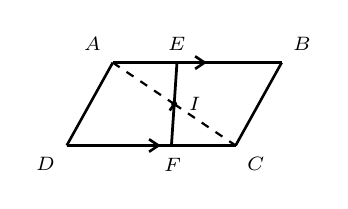
\begin{tikzpicture}[scale=0.78, every node/.style={font=\scriptsize}]
    \coordinate (D) at (0,0); \coordinate (C) at (2.75,0);
    \coordinate (A) at (0.75,1.35); \coordinate (B) at (3.50,1.35);
    \coordinate (I) at ($(A)!0.5!(C)$);
    \coordinate (E) at ($(A)!0.38!(B)$); \coordinate (F) at ($(C)!0.38!(D)$);
    \draw[line width=0.95pt, par1] (A)--(B); \draw[line width=0.95pt, par1] (D)--(C);
    \draw[line width=0.95pt] (D)--(A) (C)--(B);
    \draw[line width=0.8pt, dashed, tk1] (A)--(I) (I)--(C);
    \draw[line width=1.0pt] (E)--(F);
    \fill (I) circle (1.4pt) node[right=2pt] {$I$};
    \node[above=1pt] at (E) {$E$}; \node[below=1pt] at (F) {$F$};
    \node[above left=1pt] at (A) {$A$}; \node[above right=1pt] at (B) {$B$};
    \node[below right=1pt] at (C) {$C$}; \node[below left=1pt] at (D) {$D$};
  \end{tikzpicture}
  \end{center}
  ក្នុង $\tri{IAE}$ និង $\tri{ICF}$ មាន៖\par
  ១. $\ang{IAE} = \ang{\dotline{1.1cm}}$ (ឆ្លាស់ក្នុងនៃ $AB\parallel CD$, ហេតុផល \cnum{1})\par
  ២. $IA = \dotline{1.1cm}$ (ព្រោះ $I$ ជាផ្ចិតឆ្លុះ, ហេតុផលលេខ \dotline{0.9cm})\par
  ៣. $\ang{AIE} = \ang{\dotline{1.1cm}}$ (មុំទល់កំពូល) $\Rightarrow \tri{IAE}\cg\tri{ICF}$ (\dotline{1.2cm}) $\Rightarrow IE=IF$ ។ \\
  \hline
\end{tabular}}

% --- E5 Evaluate ---
\secbar{ផ្នែកទី៥ ៖ លំហាត់ប្រតិបត្តិ ផ្ទៀងផ្ទាត់ជាដៃគូ និង \enbf{Exit Check (E5 -- Evaluate)}}{១០ នាទី}
\textbf{ក. លំហាត់ប្រតិបត្តិ៖} ប្រលេឡូក្រាម $MNPQ$ មានផ្ចិត $O$, $MN = 3y - 1\unit{cm}$, $QP = 14\unit{cm}$, $MO = 4.5\unit{cm}$ និង $\ang{M} = 72^\circ$ ។\par\vspace{3pt}
\begin{tabular}{@{}L{13.15cm} C{5.65cm}@{}}
  ១. រកតម្លៃ $y$ (ភ្ជាប់លេខហេតុផល)៖ \dotline{7.5cm}\par\vspace{4pt}
  ២. គណនារង្វាស់មុំ $\ang{P}, \ang{N}, \ang{Q}$៖ \dotline{8.0cm}\par\vspace{4pt}
  ៣. គណនាប្រវែងអង្កត់ទ្រូង $MP$៖ \dotline{8.0cm}\par\vspace{4pt}
  ៤. \textbf{បិទបញ្ហាជន្ទល់កន្ត្រៃ E1៖} កូនជាង \dotline{1.1cm} ត្រឹមត្រូវ ព្រោះ \dotline{5.2cm}
  &
  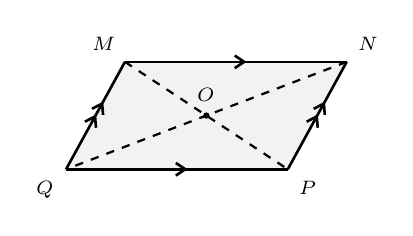
\begin{tikzpicture}[scale=0.88, baseline={(0,1.45)}, every node/.style={font=\scriptsize}]
    \coordinate (Q) at (0,0); \coordinate (P) at (3.2,0);
    \coordinate (M) at (0.85,1.55); \coordinate (N) at (4.05,1.55);
    \coordinate (O) at ($(M)!0.5!(P)$);
    \fill[gray!10] (M)--(N)--(P)--(Q)--cycle;
    \draw[line width=0.95pt, par1] (M)--(N); \draw[line width=0.95pt, par1] (Q)--(P);
    \draw[line width=0.95pt, par2] (Q)--(M); \draw[line width=0.95pt, par2] (P)--(N);
    \draw[line width=0.8pt, dashed] (M)--(P) (N)--(Q);
    \fill (O) circle (1.3pt) node[above=1.5pt] {$O$};
    \node[above left=1pt] at (M) {$M$}; \node[above right=1pt] at (N) {$N$};
    \node[below right=1pt] at (P) {$P$}; \node[below left=1pt] at (Q) {$Q$};
  \end{tikzpicture}
\end{tabular}

\vspace{5pt}
\begin{tcolorbox}[enhanced, sharp corners, colback=panelgray, colframe=black, boxrule=0.8pt, top=4pt, bottom=4pt, left=6pt, right=6pt]
  \textbf{ខ. សំណួរត្រួតពិនិត្យរហ័ស (\en{Exit Check} — គូសរង្វង់ចម្លើយត្រឹមត្រូវតែ ១)៖}\par
  ក្នុងប្រលេឡូក្រាម $ABCD$ បើមុំពីរជាប់គ្នាមានរង្វាស់ $\ang{A} = 3x + 10^\circ$ និង $\ang{B} = 2x - 5^\circ$ តើតម្លៃ $x$ ស្មើប៉ុន្មាន?\par\vspace{2pt}
  \hspace*{0.5cm}\textbf{A.} $x = 15^\circ$ \hspace{2.1cm} \textbf{B.} $x = 35^\circ$ \hspace{2.1cm} \textbf{C.} $x = 37^\circ$ \hspace{2.1cm} \textbf{D.} $x = 70^\circ$
\end{tcolorbox}

% --- Step 5 Homework ---
\secbar{ផ្នែកទី៦ ៖ កិច្ចការផ្ទះ និងបណ្ដាំផ្ញើ \enbf{(}សៀវភៅគោល ទំព័រ ១៨៥\enbf{)}}{ធ្វើក្នុងសៀវភៅកិច្ចការផ្ទះ}
$\bullet$ \textbf{លំហាត់ទី១ (លំហាត់ទី៥ ទំព័រ ១៨៥)៖} បើមុំមួយនៃប្រលេឡូក្រាមស្មើ $(2x + 20^\circ)$ ហើយមុំតគ្នាមួយទៀតស្មើ $(x - 50^\circ)$ ចូរគណនាតម្លៃ $x$ និងមុំទាំងបួន ។\par\vspace{2pt}
$\bullet$ \textbf{លំហាត់ទី២ (លំហាត់ទី៧ ទំព័រ ១៨៥ — ផ្នែកទី១)៖} ប្រលេឡូក្រាម $ABCD$ មានផ្ចិត $O$ ។ បន្ទាត់ $d$ កាត់តាម $O$ ជួប $AB, CD$ ត្រង់ $A', C'$ និងបន្ទាត់ $\Delta$ កាត់តាម $O$ ជួប $BC, AD$ ត្រង់ $B', D'$ ។ ចូរបង្ហាញថា $OA'=OC'$ និង $OB'=OD'$ រួចអានជាមុន \textbf{ទ្រឹស្ដីបទទី៤--៧} (ទំ.១៧១--១៧៤) ។

\end{document}
